\section{Topological Insulators}
\label{sec:intro:TI}


The idea of describing the physical properties of crystals with topological concepts comes from the development of understanding the quantum Hall effect (QHE). Discovered by Klaus von Klitzing~\cite{Klitzing1980}, the Hall signal of a high-mobility two-dimensional electron gas (2DEG) at low temperatures displays plateaus at $\sigma_{xy}=ne^2/h$ (where $h$ is the Planck constant) when a strong magnetic field is applied. Such plateaus happen when the two-dimensional (2D) Fermi energy $E_F$ lies between the quantized Landau levels (LLs). Although there are no itinerant states in the gap between the Landau levels in the 2D bulk, the increasing LL energy at the edge caused by the surface potential leads to states intersecting the Fermi level. Since such edge states cannot be scattered into the bulk, they provide dissipationless chiral channels for the electrons. The theoretical advances thereafter then showed that each LL in QHE has a Chern number $\nu=1$ and it lead to the development of the topological band theory. Thus QHE provides an important early example for the necessity of topological orders in describing properties of Bloch electrons.

Both the QHE and the later discovered fractional quantum Hall effect (FQHE) only exist in a strong magnetic field when the TR symmetry is broken. Then a question arises as whether the similar states could exist without a magnetic field. In 1988, the pioneering work by Haldane~\cite{Haldane1988} constructs such a model without breaking the time reversal symmetry (TRS) globally. But this model still needs a local magnetic field that points up and down at different sites. Enlightened by Haldane's work, Zhang et. al.~\cite{Bernevig06} found in 2006 that the spin-orbit coupling (SOC) could play the role of the flipping magnetic field in real solids. They also predicted that the HgTe/CdTe quantum well could be an example of the model and it was later realized experimentally by Molenkamp group~\cite{Konig2007}. This becomes the first example for the 2D TI and it's also called quantum spin Hall effect (QSHE). 


%here needs better explanation and a figure
A simple picture of QSHE is to view it as two stacking sets of QHE with counter-flowing edge states (Fig. \ref{QSHE}). The QSHE thus has two edge states which form the time-reversal partner of each other. Since the spin of the edge state is locked to its momentum in QSHE, such edge channel lacks the 2$k_F$ scattering and it leads to the quantized conductivity in Ref ~\cite{Konig2007}. Since the 2$k_F$ scattering usually contributes a significant amount to the scattering processes in transport experiments, an electric device based on QSHE is predicted to produce less Joule heating due to the decreased scattering. 
%A key player in realizing the quantum spin Hall phase is the band inversion induced by the SOC in HgTe, which later also plays a critical role in generating the 3D TIs. 
\begin{figure}[htb]
  \begin{center}            
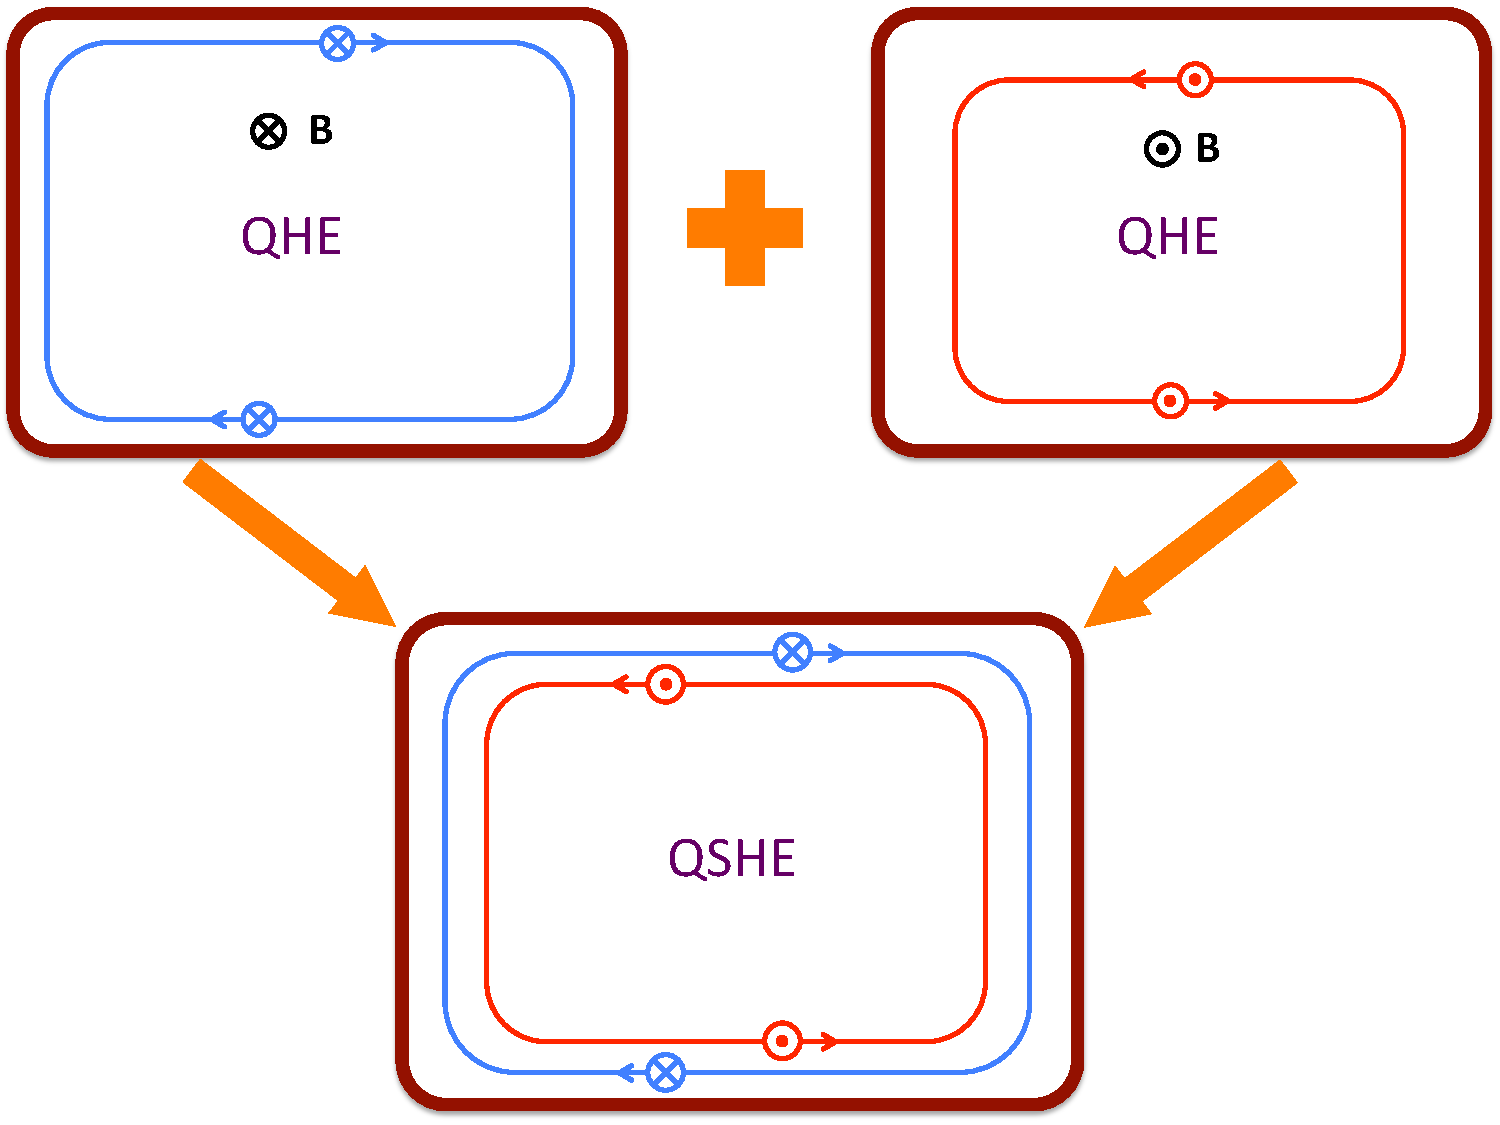
\includegraphics[width=0.9\linewidth]{ch-intro/figures/QSHE.pdf} 
\caption{\label{QSHE} (Color online) 
The edge states in quantum spin Hall effect can be viewed as a stack of two quantum Hall edge states with opposite directions.
} 
  \end{center}
\end{figure}

An important progress later is to extend the topological band theory to the 3D case. In 2007, Fu and Kane~\cite{FuKane07, Fu07} successfully made this step and found the theoretical ingredients for 3D $Z_2$ TIs. They found that four $Z_2$ topological invariants $[\nu_0; \nu_1, \nu_2, \nu_3]$ could be used to classify the different topological properties of a crystal. Within these four numbers, $[\nu_0]$ is the strong topological invariant, which is also the most important one that defines a strong or weak TI. $[\nu_1, \nu_2, \nu_3]$ are called weak topological invariants, and could be used to classify different weak TIs. Fu and Kane~\cite{FuKane07} used the pfaffians at the Kramers points inside the first Brillouin zone to calculate $[\nu_0]$ as the following:
\be
(-1)^{\nu_0}=\prod \delta_a, 
\label{eq:nu0}
\ee
where $\delta_a = Pf[\omega(\Lambda_a)]/\sqrt{Det[\omega(\Lambda_a)]} = \pm1$. Here $Pf[\omega(\Lambda_a)]$ is the pfaffian, and the $
\omega$ matrix is $\omega_{mn}(\bf k) = \Braket{u_{m -k}|\Theta|u_{nk}}$, where $\Theta$ is the time reverse operator. As a result, a 
conventional trivial insulator has topological invariants $[\nu_0; \nu_1, \nu_2, \nu_3] = [0, 0, 0, 0]$. For a strong TI, $\nu_0=1$. A weak TI has $\nu_0=0$ but at least one of the weak topological invariants is non-zero.

\begin{figure}[htb]
  \begin{center}            
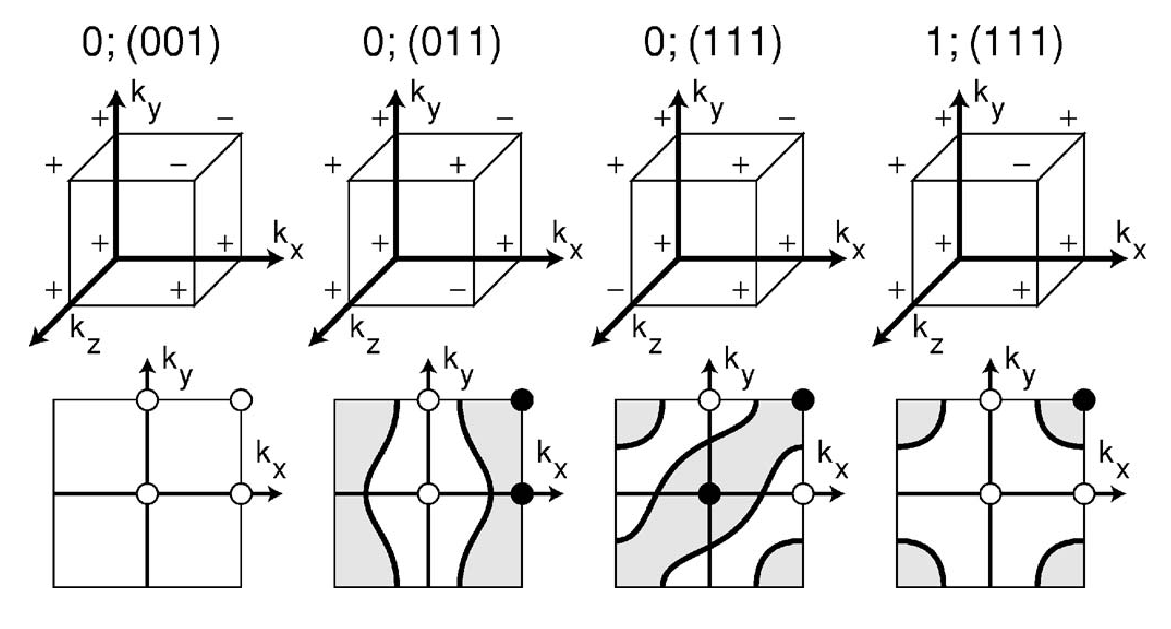
\includegraphics[width=0.9\linewidth]{ch-intro/figures/TI_class.pdf} 
\caption{\label{TI_class} (Color online) 
The four diagrams give examples of different types of weak and strong TIs. The top panels depict the signs of $\delta_i$ at the Cramers points $\Lambda_i$ in the reciprocal lattice. The bottom panels display the corresponding surface states.
} 
  \end{center}
\end{figure}

Same as the earlier found topological phases, a 3D TI also has metallic states on its edge, the 2D surface, while its 3D bulk is an insulator. These surface states also provide an easy way to distinguish strong TIs, weak TIs and trivial insulators in experiments. Fu and Kane pointed out that on the surface of a strong TI, there is an odd number of states connecting the bulk conduction band and the valence band. These surface states, which exist on every plane cleaved out of the crystal, are robust because they cannot be destroyed by local perturbations from the impurities. However, weak TIs only have some robust surface states on certain cleavage planes. By contrast, a trivial insulator do not have such robust surface states at all. Besides, one important property of the surface states on a strong TI is the spin-orbit lock-in effect. Thus, the spin direction of the surface state is always perpendicular to both the wavevector $\bf k$ and the surface normal vector $\bf{\hat{n}}$.

The prediction of the spin-polarized surface states on 3D TI has largely expanded the scope of possible experiments on the topological properties of solids. Most of the experiments are focused on strong TI, and there has been important progress in experiments with techniques like angle-resolved photoemission spectroscopy (ARPES), scanning tunneling microscopy (STM) and transport measurement. The first experimental discovery of a 3D TI is the ARPES result on Bi$_{1-x}$Sb$_x$ by Hasan's group \cite{Hsieh08, Hsieh09}. As shown in Fig. \ref{ARPES_STM}A, there are five surface bands inside the bulk band gap. The spin ARPES data showed that these surface states indeed are spin-polarized. Then more ARPES experiments found that Bi$_2$Se$_3$ and Bi$_2$Te$_3$ \cite{Xia09, Chen09} are also strong TIs but they have a much simpler surface band structure. As shown in Fig. \ref{ARPES_STM}B and D, both Bi$_2$Se$_3$ and Bi$_2$Te$_3$ only have one surface state across the bulk band gap. Since these surface states have a linear dispersion to the first order, they could be described by the Dirac equation and are also called Dirac surface states. They are also a good analog to the Dirac states in graphene. STM experients by Yazdani group\cite{Pedram09} have also confirmed the lack of back-scattering of the topological surface states. 

\begin{figure}[htb]
  \begin{center}            
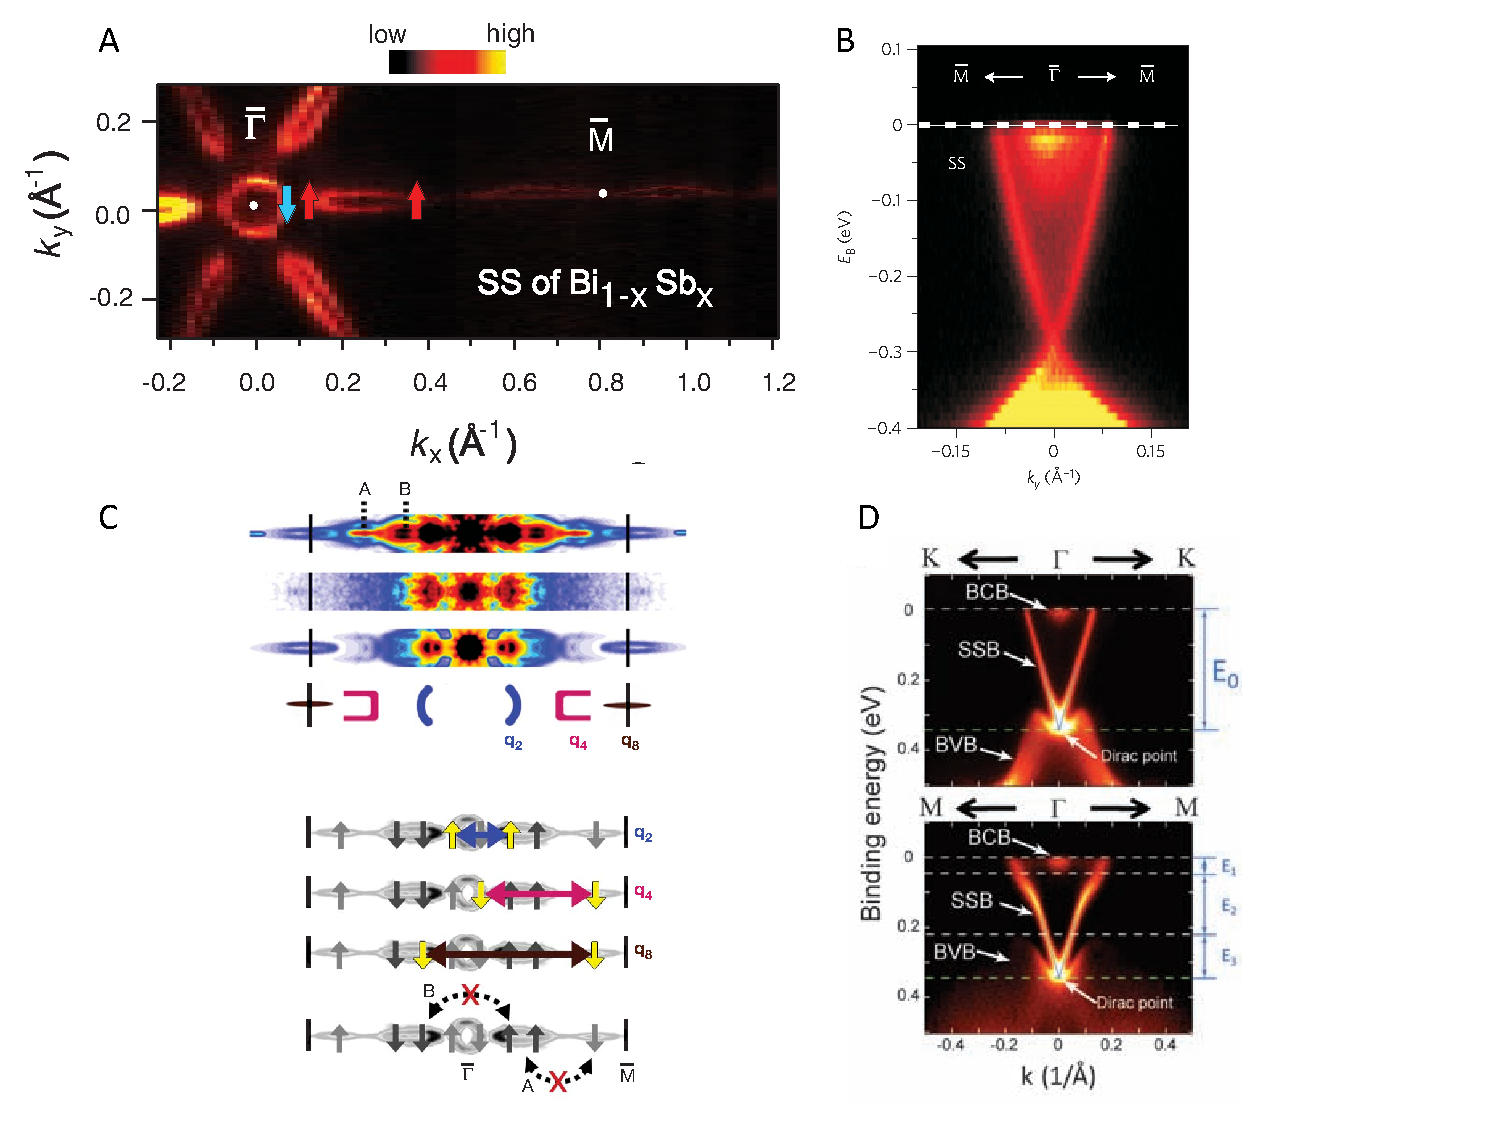
\includegraphics[width=0.9\linewidth]{ch-intro/figures/ARPES_STM.pdf} 
\caption{\label{ARPES_STM} (Color online) 
The first ARPES and STM results on some topological insulators. (A) The ARPES experiment on the first example of a strong TI, Bi$_{1-x}$Sb$_x$, indicates five spin-polarized surface states at the Fermi level\cite{Hsieh09}. (B) The ARPES data on Bi$_2$Se$_3$ shows a single surface cone with a 0.3 eV bulk energy gap \cite{Xia09}.  (C) The quasiparticle interference results in an STM experiment on Bi$_{1-x}$Sb$_x$ confirms the lack of back-scattering of the topological surface states. (D) The ARPES data on Bi$_2$Te$_3$ gives another example of a TI with a single surface cone and a large bulk energy gap \cite{Chen09}.
} 
  \end{center}
\end{figure}

Despite the fast advances in experiments using surface-sensitive techniques, the transport measurement of a TI's surface states have been difficult, mainly due to the vast amount of carriers in the bulk. Unexpected by the theory, the inverted bulk band gap induced by the SOC in TIs may still have a lot of states inside. The reason is that the crystal defects and imperfection in real TI crystals can easily dope the materials and make the as-grown crystals $n$-type (Bi$_2$Se$_3$) or $p$-type (Bi$_2$Te$_3$). Besides, the surface states are still vulnerable possibly due to the chemical reaction that happens when the sample is exposed to air. Hence, the surface states typically contribute only to a small portion of the total current, and thus are hard to detect in transport experiments. Despite the difficulty, Qu et. al. ~\cite{Qu} and Analytis et. al. ~\cite{Analytis} found the first convincing transport signals for the surface states on TI in Bi$_2$Te$_3$ and (Bi$_{1-x}$Sb$_x$)$_2$Se$_3$. These experiments have triggered enormous interest in the transport experiments on TIs. And we will discuss our progress in the transport investigation of TIs in later chapters. 

\begin{figure}[htb]
  \begin{center}            
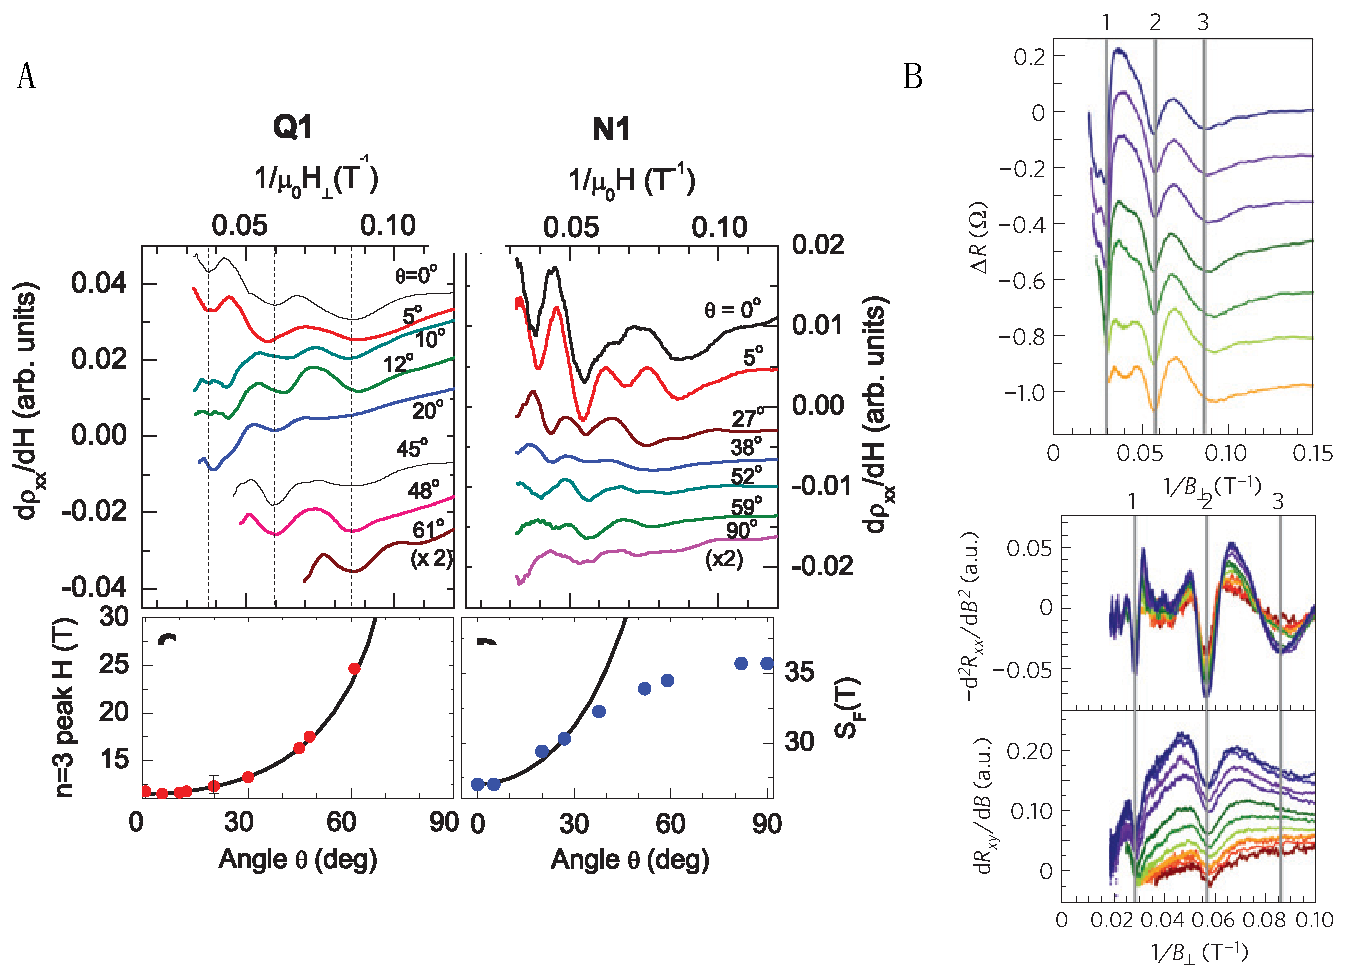
\includegraphics[width=0.9\linewidth]{ch-intro/figures/TI_transport.pdf} 
\caption{\label{TI_transport} (Color online) 
Quantum oscillations at high magnetic fields confirm the existence of high-mobility surface states on TI. (A) The different angle dependences of the quantum oscillations in nonmetallic and metallic Bi$_2$Te$_3$ samples indicate the surface origin of the quantum oscillations in nonmetallic samples. (B) Quantum oscillations in the magnetoresistance data of (Bi$_{1-x}$Sb$_x$)$_2$Se$_3$ are consistent with the behavior of surface states when the magnetic field is tilted.
} 
  \end{center}
\end{figure}


